%!TEX ROOT = thesis.tex
\chapter{LITERATURE REVIEW}
\label{chapter: 2}

This chapter would cover the literature review part of this project. This chapter would present the discussion about the datasets reviewed for this project,the semantic segmentation methods using traditional ML methods and its limitations, past work semantic segmentation using Convolutional Neural Network (CNN) and Transformer.   
\section{Satellite Images Datasets}

\FloatBarrier
\begin{landscape}
\begin{table}[]
\begin{tabular}{|c|c|c|c|c|c|c|}
\hline
\textbf{Dataset}                                                      & \textbf{Source}                                                & \textbf{\# Samples} & \textbf{\# Classes} & \textbf{Size (px)} & \textbf{Res (m)} & \textbf{Band}                                      \\ \hline
\begin{tabular}[c]{@{}c@{}}Benin Cashew \\ Plantation\end{tabular}    & Airbus Pléiades                                                & 70                  & 6                   & 1,122x1,186        & 10               & MSI                                                \\ \hline
\begin{tabular}[c]{@{}c@{}}Cloud Cover \\ Detection\end{tabular}      & Sentinel-2                                                     & 22,728              & 2                   & 512x512            & 10               & MSI                                                \\ \hline
\begin{tabular}[c]{@{}c@{}}Kenya Crop \\ Trade\end{tabular}           & Sentinel-2                                                     & 4,688               & 7                   & 3,035x2,016        & 10               & MSI                                                \\ \hline
\begin{tabular}[c]{@{}c@{}}Deep Globe \\ Land Cover\end{tabular}      & \begin{tabular}[c]{@{}c@{}}DigitalGlobe\\  +Vivid\end{tabular} & 803                 & 7                   & 2,448x2,448        & 0.5              & RGB                                                \\ \hline
DFC2022                                                               & Aerial                                                         & 3,981               & 15                  & 2,000x2,000        & 0.5              & RGB                                                \\ \hline
\begin{tabular}[c]{@{}c@{}}ETCI 2021 \\ Flood Prediction\end{tabular} & Sentinel-1                                                     & 66,810              & 2                   & 256x256            & 5–20             & SAR                                                \\ \hline
GID-15                                                               & Gaofen-2                                                       & 150                 & 15                  & 6,800x7,200        & 3                & RGB                                                \\ \hline
LandCover.ai                                                          & Aerial                                                         & 10,674              & 5                   & 512x512            & 0.25–0.5         & RGB                                                \\ \hline
    LoveDA                                                               & Google Earth                                                   & 5,987               & 7                   & 1,024x1,024        & 0.3              & RGB                                                \\ \hline
Potsdam                                                               & Aerial                                                         & 38                  & 6                   & 4,000x4,000        & 0.02             & RGB                                                \\ \hline
Vaihingen                                                             & Aerial                                                         & 33                  & 6                   & 1,281–3,816        & 0.09             & RGB                                                \\ \hline
SEN12MS                                                               & \begin{tabular}[c]{@{}c@{}}Sentinel-1/2, \\ MODIS\end{tabular} & 180,662             & 33                  & 256x256            & 10               & \begin{tabular}[c]{@{}c@{}}SAR,\\ MSI\end{tabular} \\ \hline
\end{tabular}
\caption{Datasets Reviewed for Semantic Segmentation Task}
\label{tab:datasets}
\end{table}
\end{landscape}

\FloatBarrier

Table \ref{tab:datasets} shows the list of dataset that were evaluated and considered for this project. Each of the dataset is made for semantic segmentation task meaning that each pixel in the dataset is labelled. All of the datasets except for Potsdam and Vaihingen can be downloaded using the TorchGeo library. 

%%Potsdam%%%
The Potsdam and Vaihingen datasets \cite{potsdam-vaihingen} are datasets made specifically for urban semantic segmentation. Both of the datasets are available upon request \href{https://www.isprs.org/education/benchmarks/UrbanSemLab/detection-and-reconstruction.aspx#VaihigenDataDescr}{here}. Although the images are not taken by satellites, a lot of literature reviewed such as \cite{unetformer}, \cite{a-novel-transformer}, \cite{multi-attention-network} and \cite{A2-FPN} train their semantic segmentation model using these datasets thus we think these merit a bit of discussions. Vaihingen dataset is composed of 33 images of the town Vaihingen, Germany using a drone camera withh near infrared sensor. The average size of the images is 20494 x 20064 pixels. Potsdam dataset is composed of 38 images of Potsdam town captured using the same drone as the one from vaihingen dataset. The average size of the tiles is also 20494 x 20064 pixels but with a smaller spatial resolution of 5 cm. Both datasets have 6 classes: impervious surfaces, buildings, low vegetation, trees, cars and clutters.  Figure \ref{fig:potsdam-image} and \ref{fig:potsdam-mask} shows a pair of an image and its corresponding mask from the Potsdam dataset while Figure \ref{fig:vaihingen-image} and \ref{fig:vaihingen-mask} show the ones from Vaihingen dataset.


\begin{figure}[!htb]
    \centering
    \begin{minipage}{0.5\textwidth}
        \centering
        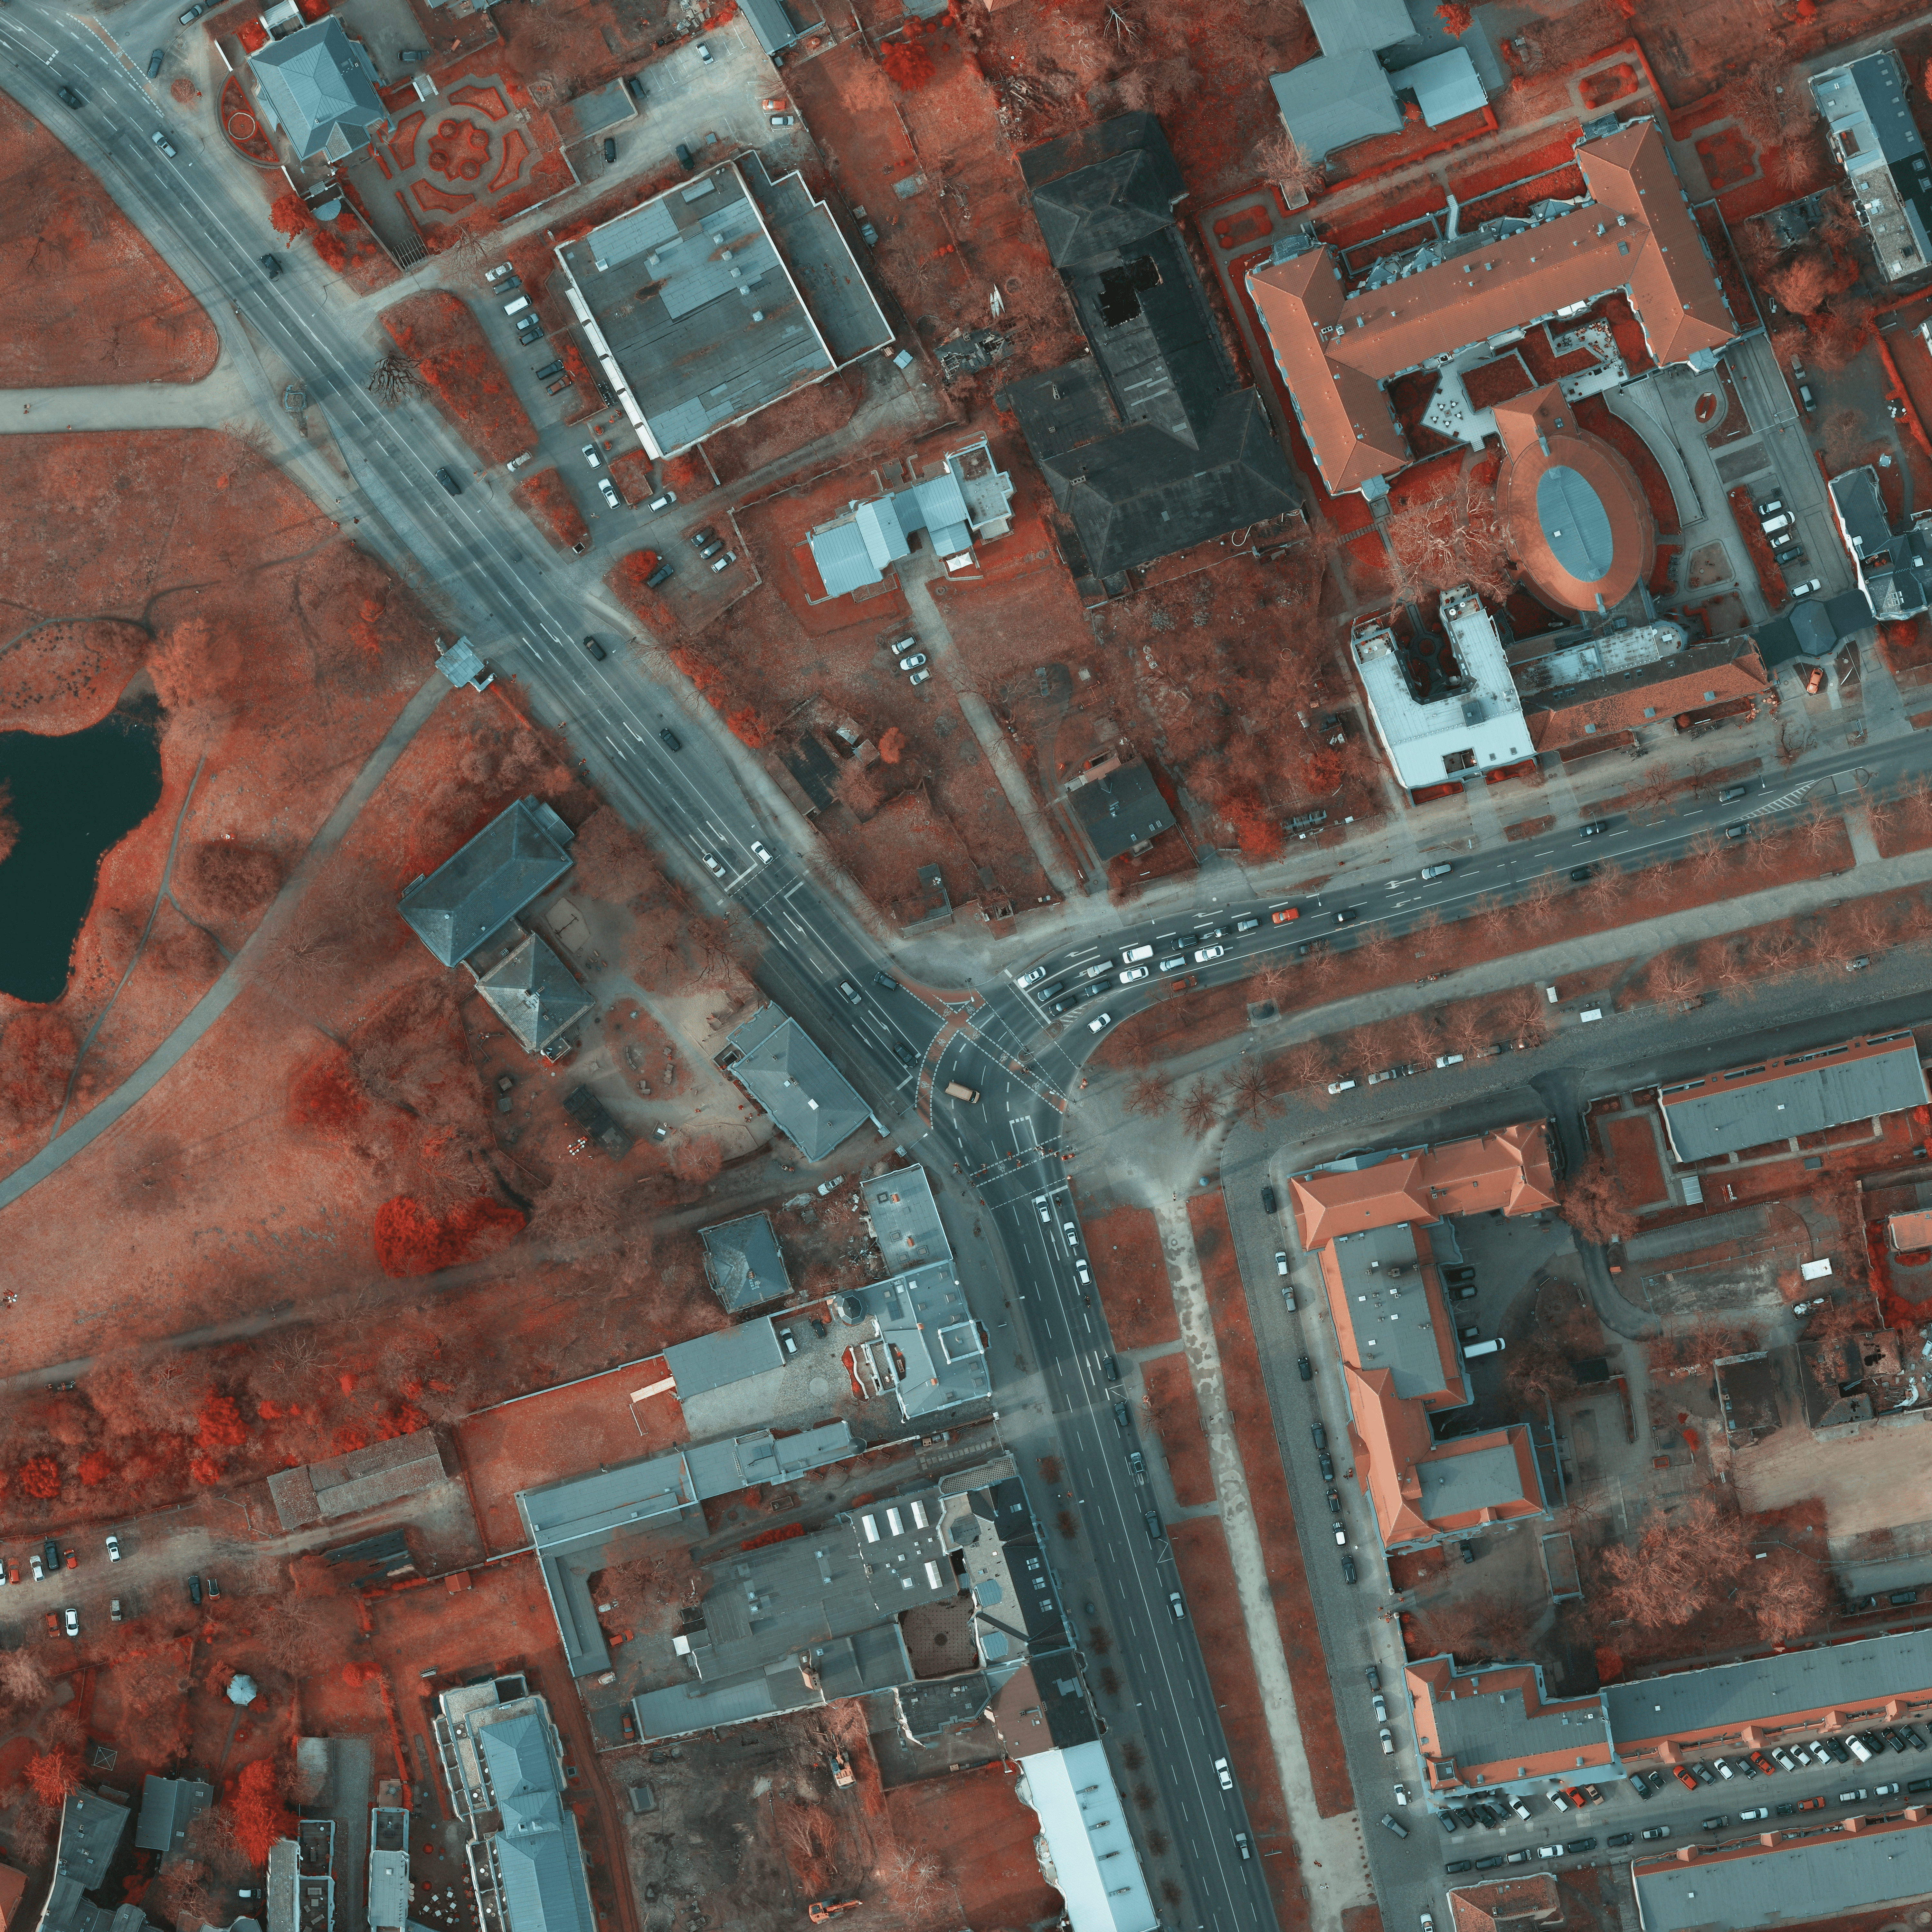
\includegraphics[width=0.95\textwidth, height=0.35\textheight]{images/potsdam-image.png}
        \caption{An Image From Potsdam Dataset \protect\cite{potsdam-vaihingen}}
        \label{fig:potsdam-image}
    \end{minipage}\hfill
    \begin{minipage}{0.5\textwidth}
        \centering
        \includegraphics[width=0.95\textwidth, height=0.35\textheight]{images/potsdam-mask.png}
        \caption{A Mask From Potsdam Dataset \protect\cite{potsdam-vaihingen}}
        \label{fig:potsdam-mask}
    \end{minipage}
\end{figure}

\begin{figure}[!htb]
    \centering
    \begin{minipage}{0.5\textwidth}
        \centering
        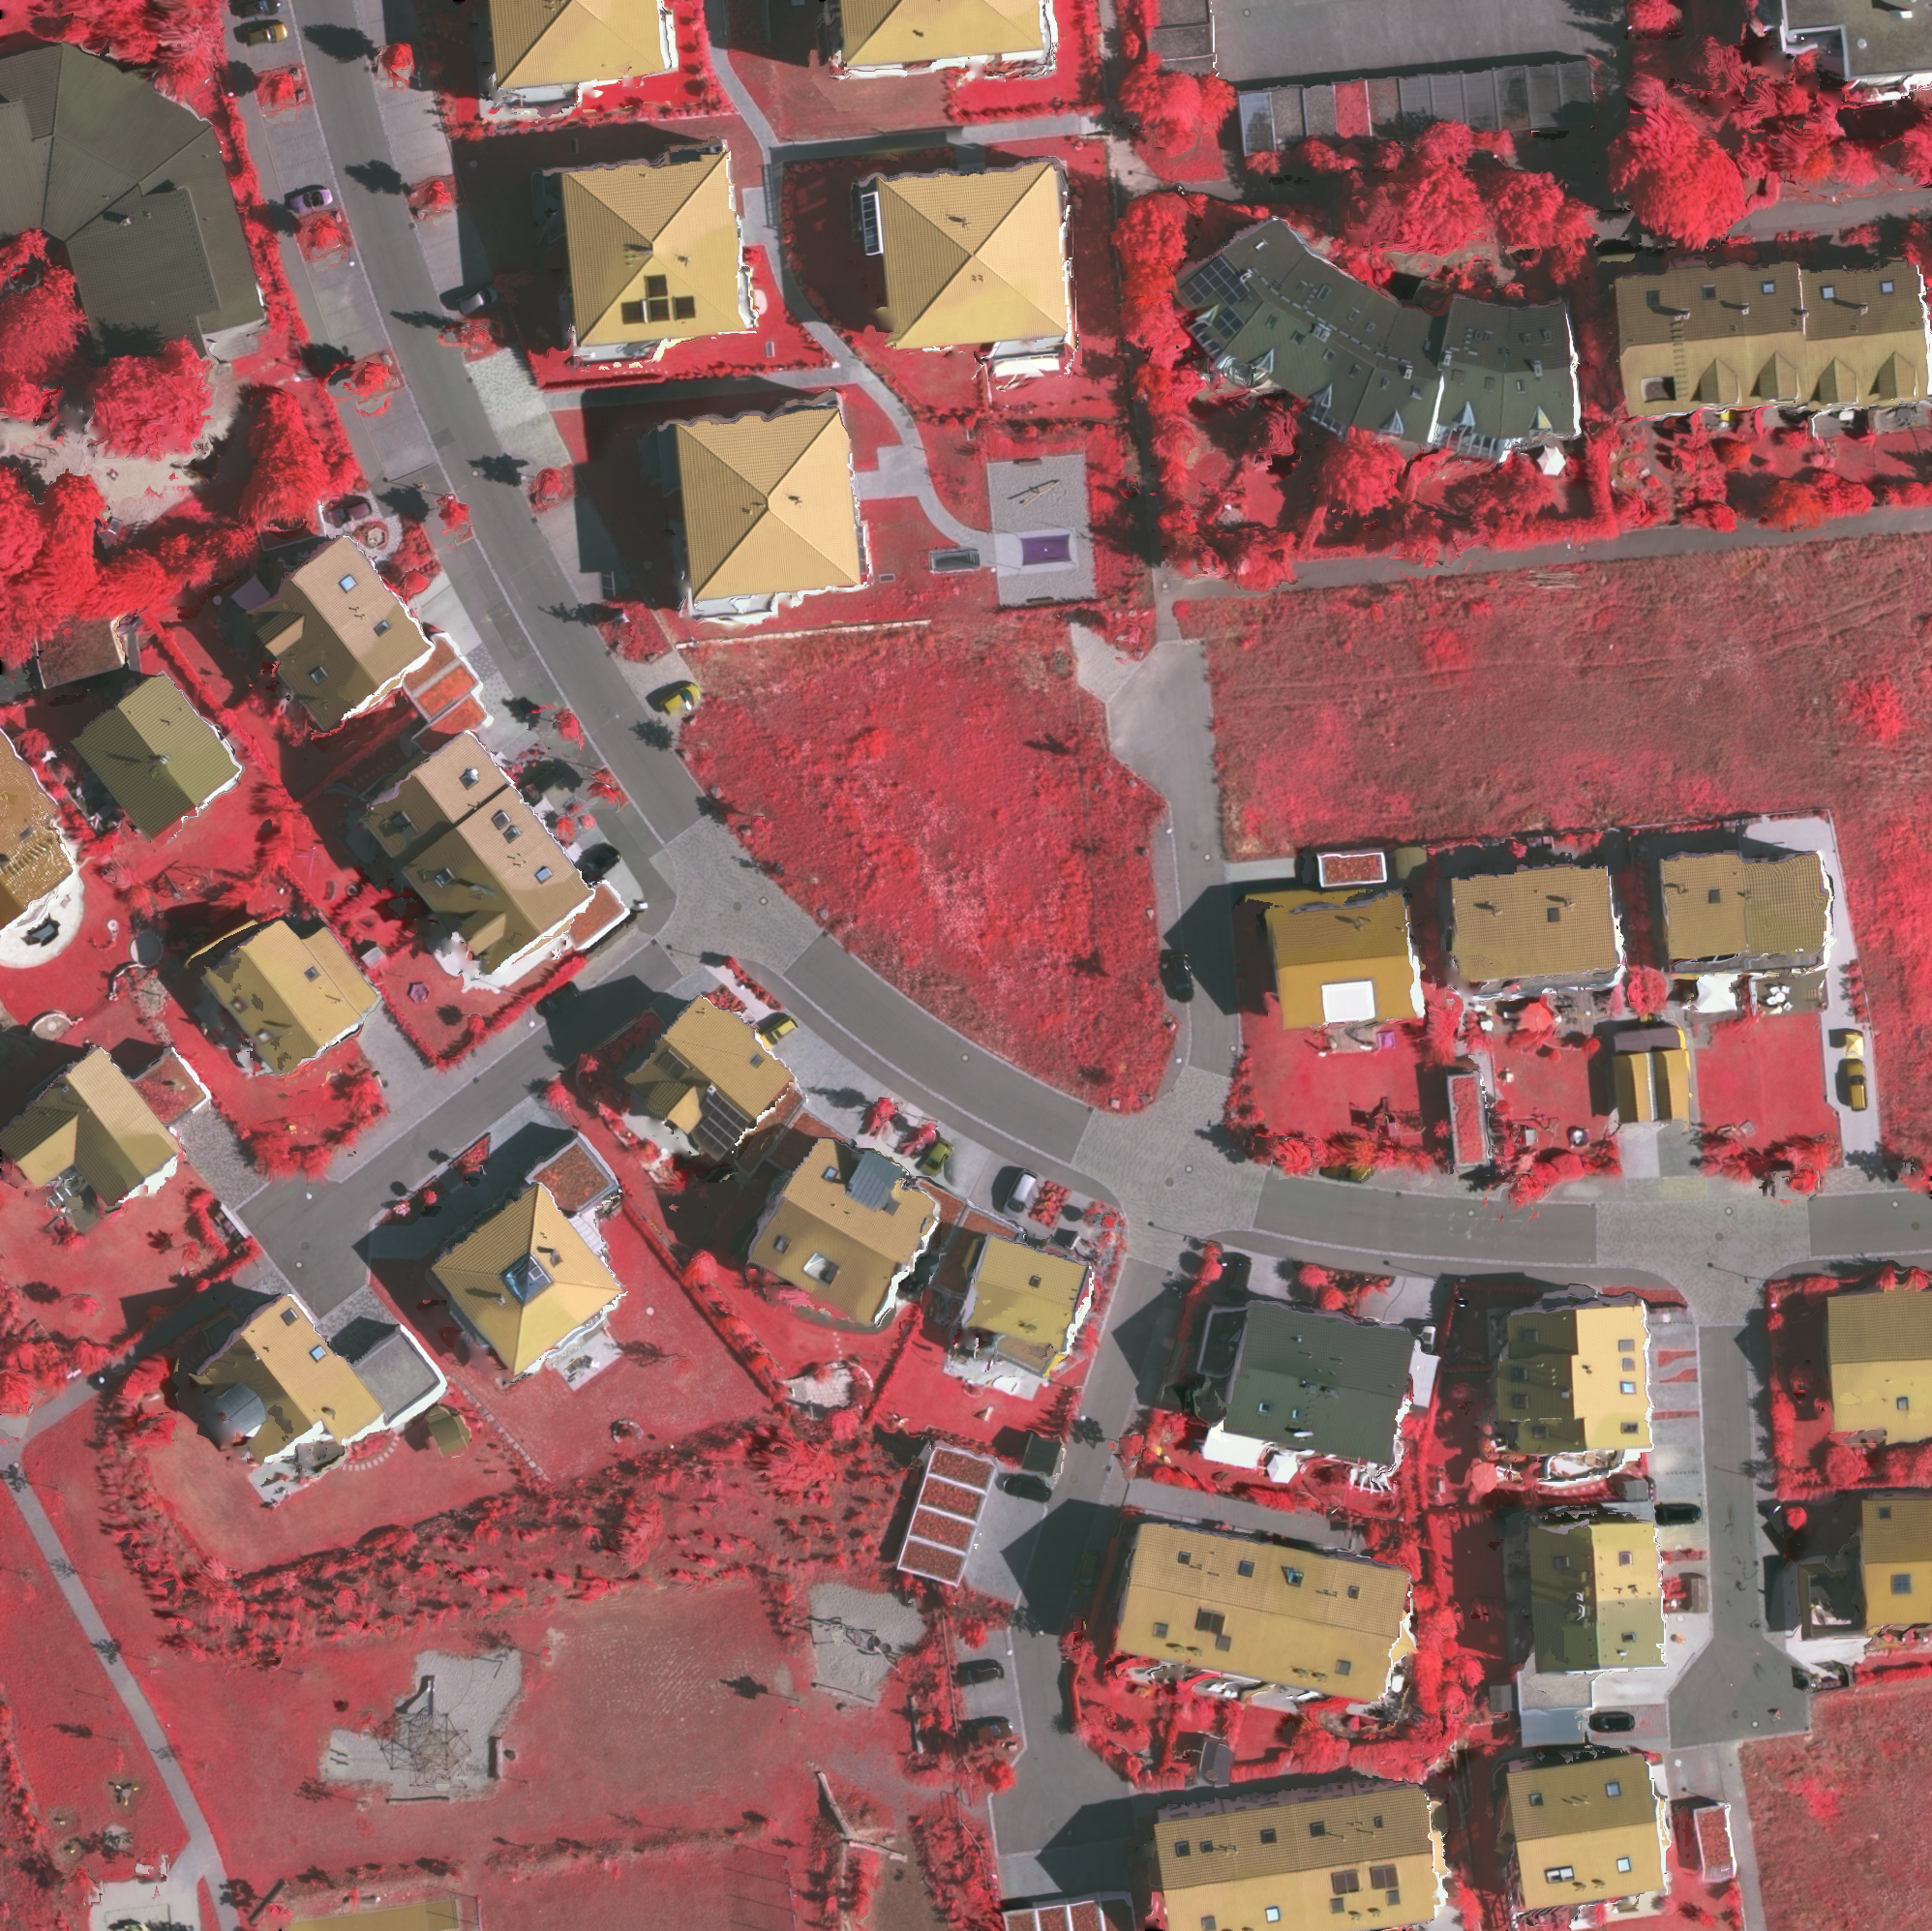
\includegraphics[width=0.95\textwidth, height=0.35\textheight]{images/vaihingen-image.png}
        \caption{An Image From Vaihingen Dataset \protect\cite{potsdam-vaihingen}}
        \label{fig:vaihingen-image}
    \end{minipage}\hfill
    \begin{minipage}{0.5\textwidth}
        \centering
        \includegraphics[width=0.95\textwidth, height=0.35\textheight]{images/vaihingen-mask.png}
\centering
\caption{A Mask From Vaihingen Dataset \protect\cite{potsdam-vaihingen}}
\label{fig:vaihingen-mask}
    \end{minipage}
\end{figure}


\FloatBarrier

%%%%%%%%%%%%%        LoveDA             %%%%%%%%

The LoveDA dataset \cite{loveda} contains 5987 High Spatial Resolution (HSR) images that are obtained from Google Earth. The images are divided into two sub-categories: urban and rural. The spatial resolution is 0.3 m, with red, green, and blue bands. After geometric registration and pre-processing, each area is covered by 1024 × 1024 images, without overlap. LoveDA dataset contains a total of 7 classes: building, road, water, agriculture, barren, forest and background. Figure \ref{fig:loveda-image} and \ref{fig:loveda-mask} shows a pair of an image and its corresponding mask from LoveDA dataset.

\FloatBarrier
\begin{figure}[!htb]
    \centering
    \begin{minipage}{0.5\textwidth}
        \centering
        \includegraphics[width=0.95\textwidth, height=0.35\textheight]{images/loveda-image.png}
        \caption{An Image From LoveDa Dataset \protect\cite{loveda}}
        \label{fig:loveda-image}
    \end{minipage}\hfill
    \begin{minipage}{0.5\textwidth}
        \centering
        \includegraphics[width=0.95\textwidth, height=0.35\textheight]{images/loveda-mask.png}
\centering
\caption{A Mask From LoveDa Dataset \protect\cite{loveda}}
\label{fig:loveda-mask}
    \end{minipage}
\end{figure}
\FloatBarrier


%%%%%%%GID%%%%%%%%%%%%
The GID-5 dataset \cite{GID2020} contains 120 6800 x 7200 HSR images with 5 classes. The classes are buildings, farms, meadow, and water. The images are obtained from Gaofen-2 satellite covering an area of more than 50,000 $km^2$. Figure \ref{fig:gid-image} and \ref{fig:gid-mask} shows an example of an image and its corresponding mask from Deep Globe dataset.

\FloatBarrier
\begin{figure}[!htb]
    \centering
    \begin{minipage}{0.5\textwidth}
        \centering
        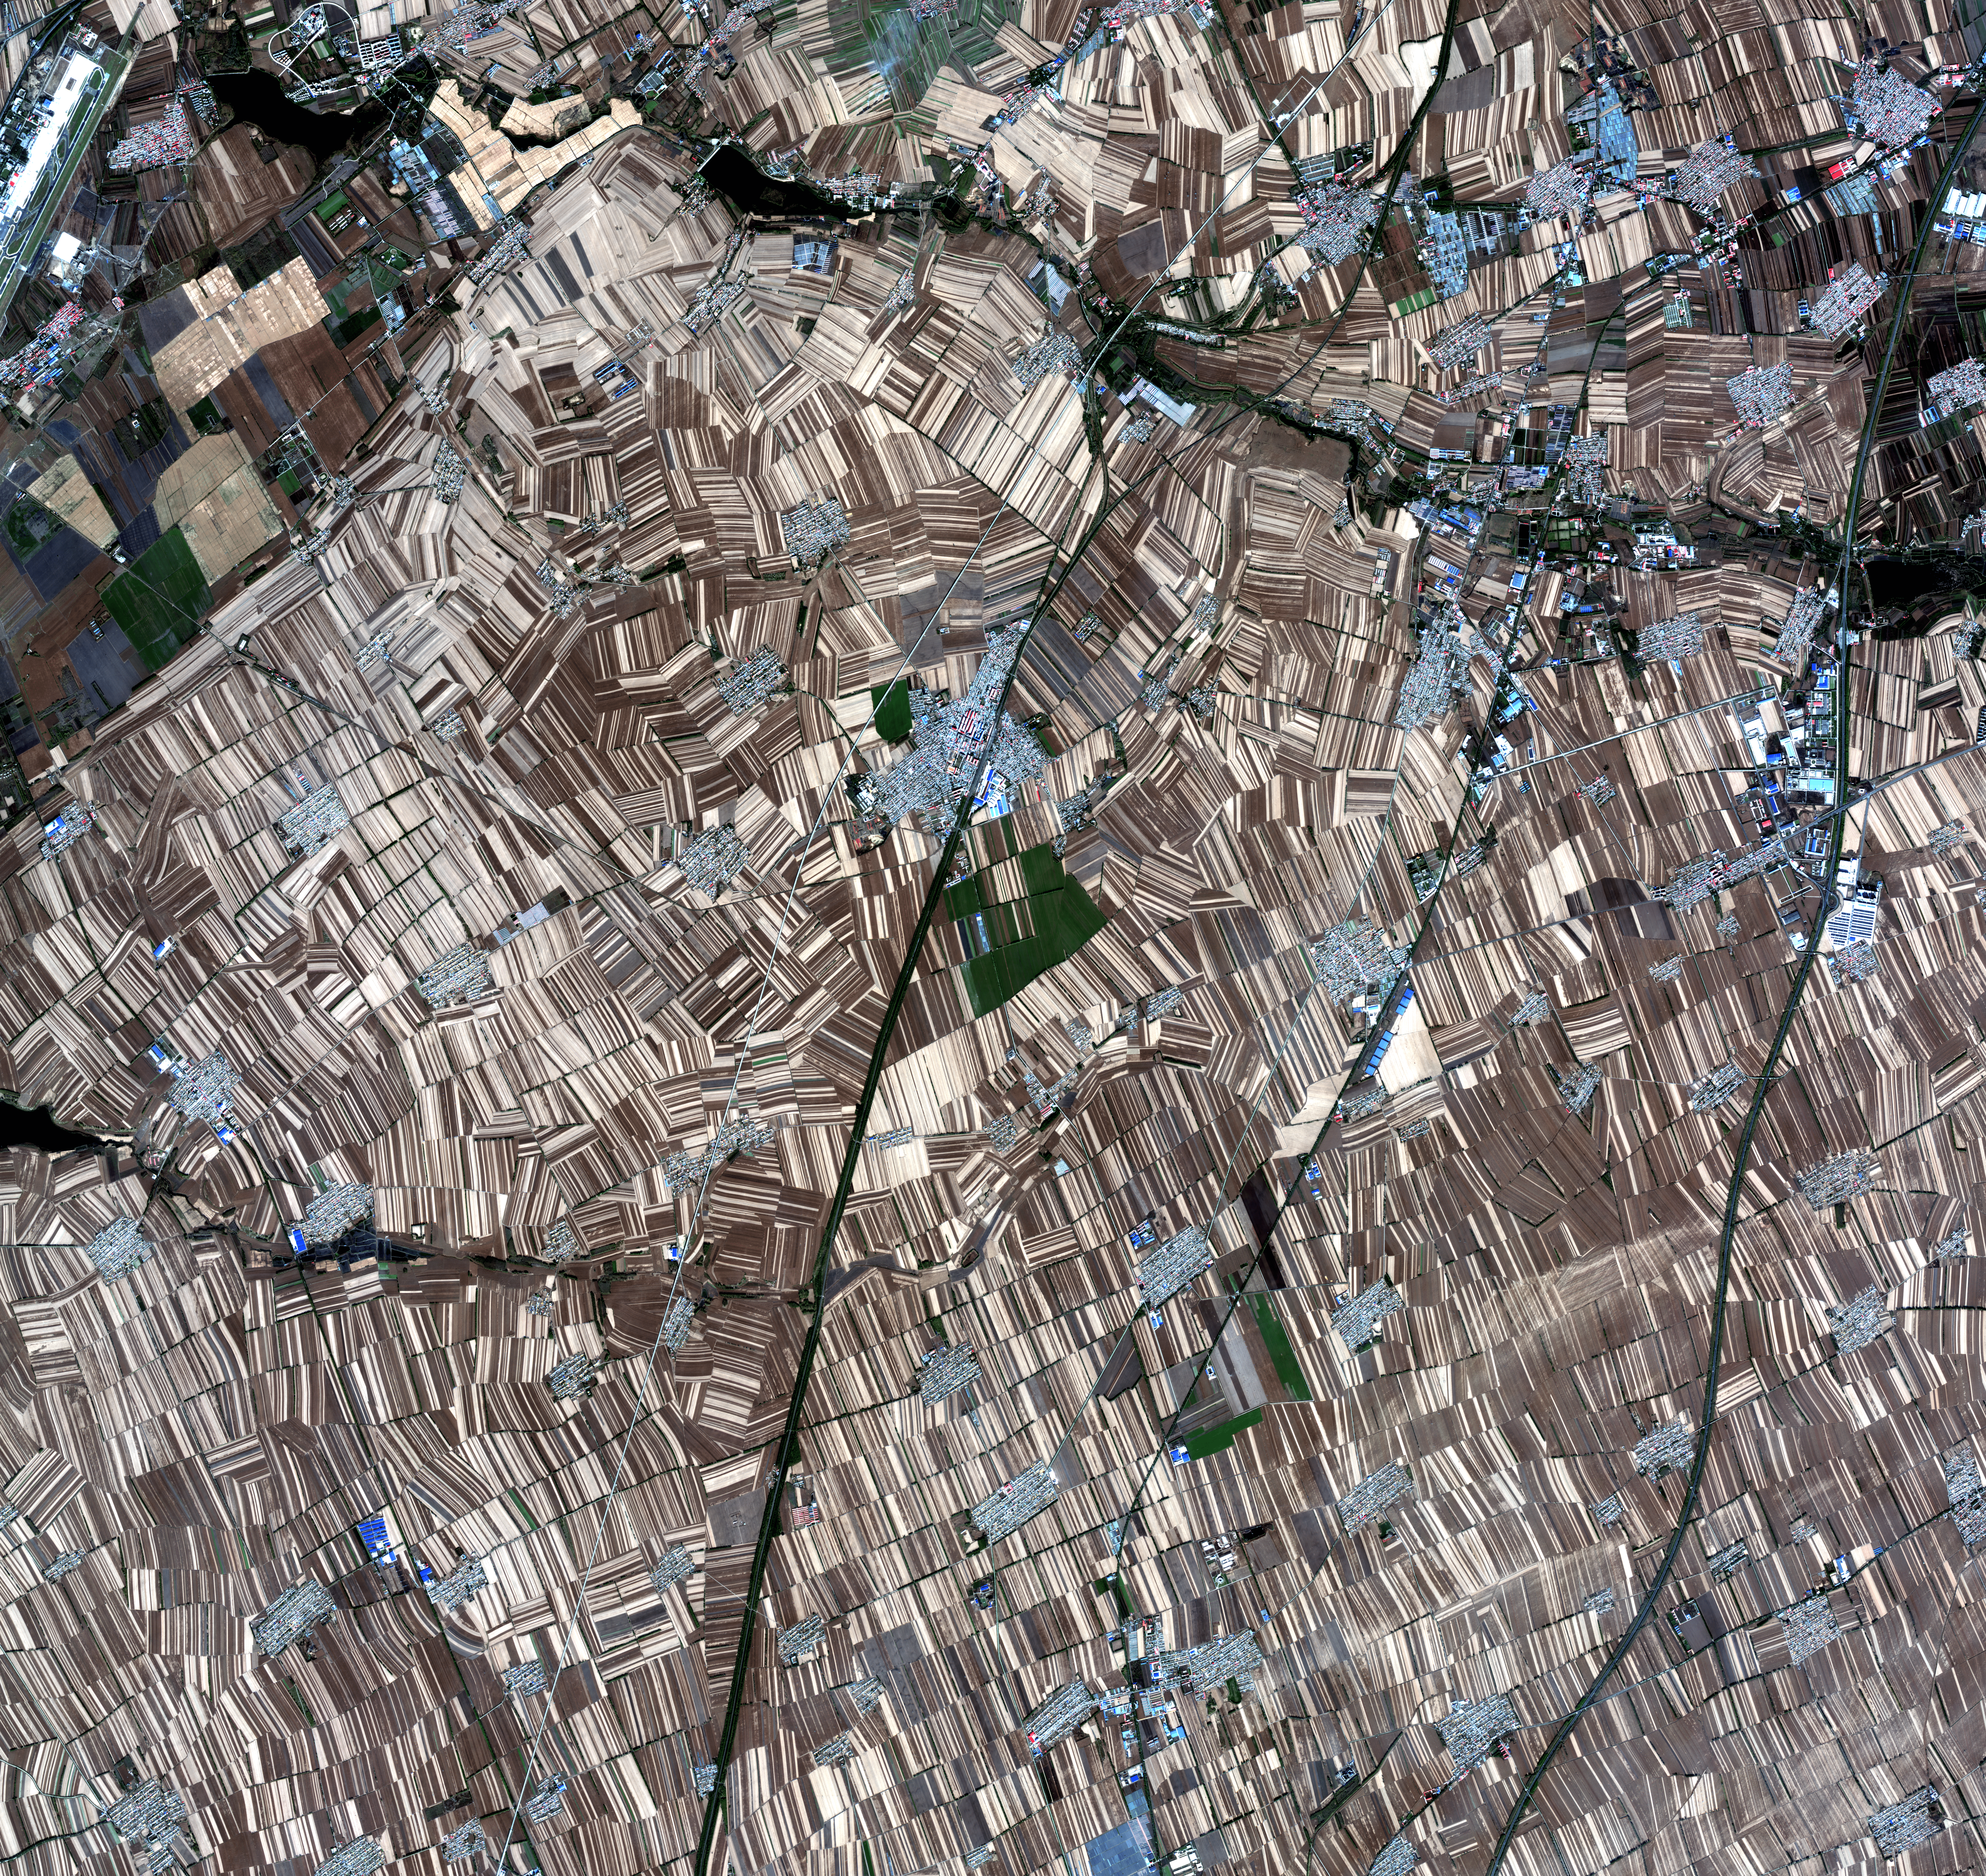
\includegraphics[width=0.95\textwidth, height=0.35\textheight]{images/gid image.png}
        \caption{An Image From GID-5 Dataset \protect\cite{GID2020}}
        \label{fig:gid-image}
    \end{minipage}\hfill
    \begin{minipage}{0.5\textwidth}
        \centering
        \includegraphics[width=0.95\textwidth, height=0.35\textheight]{images/gid mask.png}
\centering
\caption{A Mask From GID-5 Dataset \protect\cite{GID2020}}
\label{fig:gid-mask}
    \end{minipage}
\end{figure}
\FloatBarrier


%%deep-globe%%%
The Deep Globe Land Cover dataset \cite{deep-globe} contains 1146 satellite images of size 2448×2448 pixels that are split into training, validation and test sets, each with 803/171/172 images. All images are in RGB channel, with a spatial resolution of 50 cm. The segmentation masks are created by professional annotators and there are 7 total classes: urban land, agriculture, rangeland, forest, water, barren and unknown. Figure \ref{fig:deep-globe-image} and \ref{fig:deep-globe-mask} shows an example of an image and its corresponding mask from Deep Globe dataset.


\FloatBarrier
\begin{figure}[!htb]
    \centering
    \begin{minipage}{0.5\textwidth}
        \centering
        \includegraphics[width=0.95\textwidth, height=0.35\textheight]{images/deepglobe_img.jpg}
        \caption{An Image From Deep Globe Dataset \protect\cite{deep-globe}}
        \label{fig:deep-globe-image}
    \end{minipage}\hfill
    \begin{minipage}{0.5\textwidth}
        \centering
        \includegraphics[width=0.95\textwidth, height=0.35\textheight]{images/deepglobe_mask.png}
\centering
\caption{A Mask From Deep Globe Dataset \protect\cite{deep-globe}}
\label{fig:deep-globe-mask}
    \end{minipage}
\end{figure}
\FloatBarrier



The LandCover.ai dataset \cite{landcoverai} is a simple RGB-only dataset with spatial resolution of 25 (9000 × 9500 pixels) or 50 cm (4200 × 4700 pixels). There are a total of 33 images. LandCover.ai dataset has 5 classes: buildings, woodlands, water, roads and background. Figure \ref{fig:landcover-image} and \ref{fig:landcover-mask} show a pair of its image and mask.

\FloatBarrier
\begin{figure}[!htb]
    \centering
    \begin{minipage}{0.5\textwidth}
        \centering
        \includegraphics[width=0.95\textwidth, height=0.35\textheight]{images/landcoverai-image.jpg}
        \caption{An Image From Deep Landcover.ai Dataset \protect\cite{landcoverai}}
        \label{fig:landcover-image}
    \end{minipage}\hfill
    \begin{minipage}{0.5\textwidth}
        \centering
        \includegraphics[width=0.95\textwidth, height=0.35\textheight]{images/landcoverai-mask.png}
\centering
\caption{A Mask From Landcover.ai Dataset \protect\cite{landcoverai}}
\label{fig:landcover-mask}
    \end{minipage}
\end{figure}
\FloatBarrier

\section{Semantic Segmentation Before Deep Learning}

This section would elaborate on traditional methods of semantic segmentation, methods that do not apply any neural networks for semantic segmentation. Before deep learning, semantic segmentation relied heavily on feature extraction and traditional machine learning (ML) algorithm as shown in Figure \ref{fig:trad}. These two methods are rendered obsolete by deep learning.

\FloatBarrier
\begin{figure}[ht]
\includegraphics[width=5.5cm, height=7.5cm]{images/traditional.png}
\centering
\caption{Semantic Segmentation Before Deep Learning.}
\label{fig:trad}
\end{figure}
\FloatBarrier


\subsection{Feature Extraction}
Before we apply any of the traditional ML algorithm that will be discussed in the proceeding sections  we must extract the features from an image. The accuracy of traditional semantic segmentation methods heavily depends on the selected features. The features may be the numerical value of each pixel or the feature map containing the gradient of each pixel. There are three feature extraction methods discussed in this section, namely they are Histogram of Oriented Gradients, Scale-Invariant Feature Transform and Bag of Visual Words .

\begin{enumerate}
    \item \textbf{\textit{Histogram of Oriented Gradients (HOG).}} HOG features interpret any given image as a discrete function $I : \mathbb{N}^2 \rightarrow \{0...255\}$ that maps a pair value $(x,y)$ which is the coordinate of the pixel to an RGB value. Then, the partial derivative in of \(x\) and \(y\) are calculated for every pixel. The input image is now transformed into a feature map with the gradient of each pixel. Lastly, the constructed feature map is divided into smaller patches and the direction and magnitude of the histogram is calculated for each patch. \cite{DBLP:journals/corr/Thoma16a}.

    \begin{figure}[ht]
    \includegraphics[width=12cm, height=6cm]{images/hog.png}
    \centering
    \caption{An Example of Histogram of A Patch Produced by HOG}
    \label{fig:hog}
    \end{figure}
    
    \item \textbf{\textit{Scale-Invariant Feature Transform (SIFT).}} SIFT is a feature extraction algorithm that was introduced in 2004. Unlike HOG, SIFT is not affected by the orientation or scale of the input image. \cite{DBLP:journals/corr/Thoma16a}. An image will be divided into smaller patches and the difference-of-Gaussian (DoG)is calculated. Next, local extrema is searched to be be assigned as potential key points. Lastly, after the key points are discovered, an 8-bin orientation histogram is created for each patch to math the key points. The final output will be a feature map containing accepted key points. A more thorough explanation is available in the original paper \cite{SIFT}.

    \begin{figure}[ht]
    \includegraphics[width=12cm, height=7.5cm]{images/sift_keypoints.jpg}
    \centering
    \caption{Each circle represents the location and orientation of SIFT keypoints}
    \label{fig:sift_keypoints}
    \end{figure}

    
    \item \textbf{\textit{Bag of Visual Words (BOV).}} BOV construct sparse histograms that contain the frequency of features in an image. Those features are usually extracted using SIFT \cite{DBLP:journals/corr/Thoma16a}. BOV is often used alongside other feature extractors such as SIFT by assigning each SIFT descriptor to the closest entry in a visual dictionary.
\end{enumerate}

\subsection{Traditional Machine Learning Algorithm}
\subsubsection{Random Decision Forest for Semantic Segmentation}
 A decision tree is a tree where each leaf represents a class and each non-leaf nodes uses the feature inputs to decide which branch to descend to \cite{DBLP:journals/corr/Thoma16a}. A random decision tree is as decision tree that is injected with some randomness during the training phase  to reduce over-fitting and increase accuracy. Random Decision Forest is an unsupervised ensemble learning method that are made up of multiple independently constructed random decision trees. An in-depth explanation to semantic segmentation using Random Decision Forest is given by \cite{Schroff2008ObjectCS}. 
 
\subsubsection{Support Vector Machines (SVM) for Semantic Segmentation}

Support Vector Machines (SVM) works by assuming that the data is linearly separable, SVM is a task of solving the optimal margin classifier:

\begin{equation}
    min_{w,b} \quad \frac{1}{2}||w||^2 \\
\end{equation}

\begin{equation}
    s.t. \quad \mathbf{y}^{i}(\mathbf{w}^T \mathbf{x}^i +\mathbf{b})\geqslant 1, i \in {1...m}
\end{equation}

\vspace{0.1cm}

Where $\mathbf{w}$ is the weight, $/mathbf{x}$ the input vector, $\mathbf{y}$ is the output vector and $\mathbf{b}$ is the bias. $\mathbf{w}$ can be defined as:

\begin{equation}
    \mathbf{w} = \sum_{i=1}^m \alpha_i \mathbf{y}_i \mathbf{x}_i
\end{equation}

Where $\alpha$ is the Lagrange multiplier.

For dataset that is not linearly separable we can transform the vector $\mathbf{x}$ into a higher dimension using a non-linear mapping $\psi$. Thus instead of learning using $\mathbf{x}$, we may learn using a higher-dimensional features generated by $\mathbf{\psi(x)}$, this method is called the \textit{kernel trick}. Specifically, given a feature mapping $\psi$, we define the corresponding kernel to be:    

\begin{equation}
    K(x,z)=\psi(x)^T\psi(z)
\end{equation}

\subsubsection{Markov Random Field (MRF)} MRF maps an image onto an undirected graph where each node is a pair of random variable $(x,y)$ assigned to each pixel and the edges connect adjacent pixels \cite{YU201882}. $x$ represents the class label of a pixel and $y$ represents the RGB value of a pixel. Which means $x$ has a range of ${0...n}$ and y has a range of ${0...255}$ with $n$ being the number of classes.  Every edge is assigned a conditional probability of $x,y$ can be expressed as:
\begin{equation}
    P(x,y) = \frac{1}{Z} e^{-E(x,y)}
\end{equation}

Where $Z = \sum_{x,y}e^{-E(x,y)}$ and it is called the partition function and $E$ is the energy function which is expressed as $E(x,y) = \sum_{c\in C}\psi_{c}(x,y)$, where $\psi$ is called the clique potential \cite{DBLP:journals/corr/Thoma16a}. A thorough presentation of MRF can be found in \cite{markovbook}. 

\subsubsection{Conditional Random Field (CRF) for Semantic Segmentation} CRF is an extension of MRF but it learns $P(x|y)$ instead of $P(x,y)$ \cite{DBLP:journals/corr/Thoma16a}. There are two advantages that CRF has over MRF. The first one being it does not to estimate the distribution of x. The second advantage is the consequence of the first one, as the distribution of x is not being estimated, less computation is required hence making CRF faster than MRF \cite{YU201882}. CRF is often used in conjunction with neural networks as a post-processing method for semantic segmentation task. It is is used to smoothen the output mask \cite{crf-semantic}.

\section{Limitations of Traditional Methods}
\begin{enumerate}
    \item The traditional method is simply less accurate. As an example the best traditional method back in 2015 which utilized SIFT and Fisher Vectors, had a 25.7\% error rate on semantic segmentation task on ILSVRC-2010 dataset. While AlexNet proposed by \cite{alexnet} had an error rate of 17.0\% \cite{DBLP:journals/corr/Thoma16a}.
    \item  Feature extraction method such as SIFT and Random Decision Forest require researchers to come up with a good hand-crafted feature to achieve high accuracy while good features are very hard to produce. Compared this with the automatically learned features provided by deep learning, traditional methods would require a lot more time and effort.

\end{enumerate}


\section{Semantic Segmentation of Satellite Images Using Convolutional Neural Networks}

Semantic segmentation task has been long dominated by Convolutional Neural network (CNN). The Fully Convolutional Network (FCN) \cite{7298965} is the first network proven to be an effective Deep Learning method method for semantic segmentation task. Altough the result seems promising, the over-simplified design  tends to produce coarse results.

To tackle this problem, better CNNs were proposed such as U-Net \cite{unet} which  introduced the encoder-decoder framework which has become the standard structure of satellite images segmentation network \cite{unetformer}. U-Net introduced two symmetric paths: a contracting path, which is also known as the encoder to extract local features, and an expanding path which is also called the decoder, for extracting position. The encoder gradually apply convolutions and max pooling to reduce the resolution of the feature map, while the decoder extracts global information by restoring the spatial resolution. At every level of the decoder skip connections are used to concatenate its output with the feature maps from the encoder of the same level. Figure \ref{fig:unet} show the U-Net architecture. Benefiting from its translation equivariance and locality, U-Net enhances the semantic segmentation performance significantly and the encode-decoder framework has been a major influence towards semantic segmentation task. 

\begin{figure}[ht]
\includegraphics[width=10.5cm, height=7cm]{images/unet.png}
\centering
\caption{U-Net Architecture \protect\cite{unet}}
\label{fig:unet}
\end{figure}

Even though the results are promising, U-Net is limited by the convolutional mechanism that is only good at processing local properties. There are two types of approaches to address this issue, either modifying the convolution layer or introducing the attention mechanism. Such examples of the first approach is to use large kernel sizes \cite{enlarge-receptive-field}, or utilising feature pyramids \cite{feature-pyramid}. Examples of the second can be found in Attentive Bilateral Contextual Network \cite{abcnet} and Attention U-Net \cite{attention-unet}.

Attention U-Net \cite{attention-unet} is a model that aims to improve U-Net by introducing attention gates in the skip connections between the encoder and decoder as shown in \ref{fig:attention-unet}. The results showed that Attention U-Net performs better than traditional U-Net for segmentation of CT scans images.

\begin{figure}[ht]
\includegraphics[width=10.5cm, height=7cm]{images/attention-unet.png}
\centering
\caption{Attention U-Net Architecture \protect\cite{attention-unet}}
\label{fig:attention-unet}
\end{figure}

U-Net with added attention mechanism is the approach favored by most literature focusing on semantic segmentation of satellite images. Multi Attention U-Net(MA-Unet) \cite{multi-attention-unet}  uses residual structure and simple attention modules. According to figure \ref{fig:maunet} the decoder in MA-Unet uses transposed convolution and attention modules at every feature fusion stage. MA-Unet performs better at segmenting classes with fine details such aeroplanes. MA-Unet has the highest mIoU on both dataset with 63.94\% on WHDLD dataset and 61.90\% on DLRSD dataset.

Spatial Attention U-Net (SA-Unet) \cite{improved-unet} uses atrous spatial pyramid pooling as its encoder and attention modules at every skip connection like we have seen in Attention U-Net.  \cite{attention-unet-road} employs U-Net with attention to extract roads from satellite images. Instead of using simple attention modules at every skip connections, they uses attention module only once at the lowest skip connection.

\begin{figure}[ht]
\includegraphics[width=10.5cm, height=7cm]{images/maunet.png}
\centering
\caption{Multi Attention U-Net Architecture \protect\cite{multi-attention-unet}}
\label{fig:maunet}
\end{figure}

\section{Semantic Segmentation of Satellite Images Using Vision Transformers}

Transformers were introduced by \cite{attention-is-all-you-need} and since its inception it has been the standard model for Natural Language Processing (NLP). Transformers that are used for computer vision are called Vision Transformers to differentiate it from its NLP counterpart. Vision Transformers essentially processes a 2 dimensional image as a 1 dimensional sequence.

%%%%%benchmarking-scaling%%%%%%%
Since its inception, there are lot of researches that aim to utilize Transformers for semantic segmentation of satellite images. 
\cite{benchmarking-scaling} did a comparison of ViT, ResNet, MLPMixer and VGG trained using the BigEarthNet dataset for semantic segmentation and they concluded that ViT with a patch size of 6 delivered a slightly better performance than the rest while consuming less time to train. Interestingly, ViT with smaller patch size has lower F scores while requiring more time to train.

%%%%%%%%%%%%%%%%%%%%%%%%%%%%%  ViT
\subsection{Vision Transformer (ViT)}
Vision Transformer from \cite{16x16} is the first group of researchers that experimented with Vision Transformer by using a standard Transformer directly with minimal modofocations to images. Their model is known as Vision Transformer (ViT) as it is the first Vision Transformer. They split an image into patches, apply linear embeddings to transform the patches into vectors that are used as an input to a Transformer. The image patches were treated the same way as word tokens do in an NLP application. This methods fails to capture the local context provided  CNNs hence it is unsuitable for semantic segmentation task. Figure \ref{fig:vit} shows the ViT architecture.
\FloatBarrier
\begin{figure}[ht]
\includegraphics[width=13.5cm, height=9cm]{images/vision transformer.png}
\centering
\caption{ViT Architecture \protect\cite{16x16}}
\label{fig:vit}
\end{figure}
\FloatBarrier

\subsection{UNetFormer}
%%unetformer
UNetFormer \cite{unetformer} proposes a UNet-like Transformer for semantic segmentation task trained using the UAVid, Vaihingen, Potsdam and LoveDA datasets.UNetFormer has the same encoder-decoder framework as the other U-Net variants. Referring to figure \ref{fig:unetformer} UNetFormer uses either a ResNet18 endcoder and a Transformer with an added global-local Transformer block (GLTB) that are used as its decoder. 

 Each stage of ResNet18's four stages involves a scale factor of 2 downsampling of the feature map, which is then combined with the features produced by the GLTB of the decoder using a weighted sum operation at every level.


\FloatBarrier
\begin{figure}[ht]
\centering
\includegraphics[width=10.5cm, height=7cm]{images/unetformer.jpg}
\caption{UNetFormer Architecture \protect\cite{unetformer}}
\label{fig:unetformer}
\end{figure}
\begin{figure}[ht]
\centering
\includegraphics[width=10.5cm, height=7cm]{images/gltb.jpg}
\caption{ Illustration of (a) the standard Transformer block and (b) the Transformer block with GLTB \protect\cite{unetformer}}
\label{fig:gltb}
\end{figure}
\FloatBarrier

The global-local attention, multi-layer perceptron, two layers of batch normalisation, and two extra processes make up the GLTB. According to Figure \ref{fig:unetformer-besar}, the global branch and the local branch make up the global-local attention. The local branch extracts the local environment using two parallel convolutional layers with kernel sizes of 3 and 1. Before performing the final sum operation, two batch normalisation processes are used. Figure 2.28 shows how the global branch captures the overall context using the same window-based multi-head self-attention as Swin Transformer.

\FloatBarrier
\begin{figure}[ht]
\includegraphics[width=13.5cm, height=18cm]{images/unetformer besar.jpg}
\centering
\caption{Cross-shaped Window Context Interaction in UNetFormer \protect\cite{unetformer}}
\label{fig:unetformer-besar}
\end{figure}
\FloatBarrier

The author developed a cross-shaped window context interaction to generate the relationship between the windows to reduce the computing compared to the Swin Transformer which uses a shifting windows mechanism. The cross-shaped window context interaction combines the two feature maps created by a horizontal average pooling layer and a vertical average pooling layer to capture the overall context. Using the horizontal average pooling layer, the relationship with any point in Window 1, $P^{m,n}_1$  with any point in Window 2, $P^{m+w,n}_2$ can be expressed as:

\begin{equation}
    P^{m,n}_1 = \frac{\sum^{w-m-1}_{i=0}P^{m+i,n}_1 + \sum^m_{j=0}P^{m+w-j,n}_2}{w}
\end{equation}
\begin{equation}
    P^{m+i,n}_1 = D_i (P^{m,n}_1)
\end{equation}
\begin{equation}
    P^{m+w-j,n}_2 = D_j(P^{m+w,n}_2)
\end{equation}

\FloatBarrier
Where w is the window size and D is its attention. Similarly, the vertical relationship between Window 1 and Window 3 can be established in a similar way.

\FloatBarrier
\begin{figure}[ht]
\includegraphics[width=10.5cm, height=7cm]{images/frh.jpg}
\centering
\caption{Feature refinement Head of UNetFormer \protect\cite{unetformer}}
\label{fig:frh}
\end{figure}
\FloatBarrier

Finally, UNetFormer uses a Feature Refinement Head (FRH) right before the output layer to provide semantic meaning. FRH received the fused feature as shown in \ref{fig:unetformer} as its input. Then, two path are constructed as shown in figure \ref{fig:frh}. The first path is called the channel path while the second path is called the spatial path. The channel path uses a global average pooling layer to generate a channel-wise attention map $\textbf{C} \in \mathbb{R}^{1\times 1 \times c}$ , where c is the channel dimension. Then two 1x1 convolutional layers are used to the channel dimension a factor of 4 and then expands it back to its original dimension. The spatial path produce as spatial-wise attention map using convolutions. The output of the two paths are concatenated before a 1x1 convolutional layer and an up sampling operation are used as post processing.

\citeA{unetformer} also experimented with the choice of the encoder by substituting the ResNet18 with a list of lightweight Vision Transformers: ViT-Tiny \cite{16x16}, Swin-Tiny \cite{swin-v1} and CoaT-Mini \cite{coat}. The results showed that by using lightweight Vision Transformers as the encoder provided very litle incrase of accuracy but  greatly reduces the inference speed as shown in Table \ref{tab:unetformer-exp}. 

\FloatBarrier
\begin{table}[!h]
\centering
\begin{tabular}{|c|c|c|c|c|}
\hline
\textbf{Encoder} & \textbf{Complexity (G)} & \textbf{Parameters (M)} & \multicolumn{1}{l|}{\textbf{Speed}} & \multicolumn{1}{l|}{\textbf{mIoU}} \\ \hline
ViT-Tiny         & 35.31                   & 8.6                     & 30.2                                & 69.1                               \\ \hline
Swin-Tiny        & 104.4                   & 28.0                    & 28.8                                & 70.6                               \\ \hline
CoaT-Mini        & 159.7                   & 10.6                    & 10.6                                & 70.5                               \\ \hline
ResNet18         & 46.9                    & 11.7                    & 115.6                               & 70.0                               \\ \hline
\end{tabular}
\label{tab:unetformer-exp}
\caption {Experiment of Different Encoders on UNetFormer}
\end{table}
\FloatBarrier

%%%LANET%%%%%%
\subsection{LANet}
Local Attention Network (LANet) \cite{lanet} introduced two additional modules to improve semantic segmentation of satellite images. The first modeule, the Patch Attention Module (PAM) enhanced the embedding of local context while  the second module, the Attention Embedding Module (AEM) enriches spatial information. Referring to Figure \ref{fig:lanet} The high-level features produced by the late layers of the CNNs will pass through a PAM to get its feature enhanced, while the low-level features produced by early layers of a CNN are first enhanced by a PAM, before being embedded with the output of AEM which contains hih-level semantic information. The final output is the fusion of the outputs from the top and bottom channels. 

\FloatBarrier
\begin{figure}[ht]
\includegraphics[width=12.5cm, height=9.5cm]{images/lanet.png}
\centering
\caption{LANet Architecture \protect\cite{lanet}}
\label{fig:lanet}
\end{figure}

\FloatBarrier

Referring to figure \ref{fig:pam}, PAM will first generate a local descriptor for each channel of every patch, $z_c$ which can be expressed as:

\begin{equation}
    z_c = \frac{1}{h_p w_p} \sum_{i=1}^{h_p} \sum_{j=1}^{w_p} x_c(i,j)
\end{equation}

where $h_p$ and $w_p$ is the horizontal and vertical size of the patch and $x_c$ is the pixel value at the $cth$ channel. In this way, a c-channel vector $z_p$ will be generated, which contains the statistics describing the patch p. 
\begin{figure}[ht]
\includegraphics[width=9.5cm, height=4.5cm]{images/pam.png}
\centering
\caption{Patch Attention Module in LANet \protect\cite{lanet}}
\label{fig:pam}
\end{figure}
\FloatBarrier

Concatenating low-level data with high-level features is the most common method employed in most networks, but this method only slightly improves performance. The authors suggested using AEM to combine high-level and low-level features without sacrificing the latter's spatial specifics. Figure \ref{fig:aem} shows the implementation of AEM. First, they generate a high-level feature descriptor map, $z_c$ and low-level descriptor map , $x_c$ using the same formula in PAM. Then, an attention map, $a_c$ is generated using average pooling, 1 x 1 convolution and up sampling. Finally $a_c$ will be added to $x_c$ to generate an improved low-level descriptor.  
\begin{figure}[ht]
\includegraphics[width=9.5cm, height=4.5cm]{images/aem.png}
\centering
\caption{Attention Embedding Module in LANet \protect\cite{lanet}}
\label{fig:aem}
\end{figure}
\FloatBarrier


%%%%%%%A Novel Transformer Based Semantic Segmentation Scheme for Fine-Resolution
\subsection{DC-Swin}
\citeA{a-novel-transformer}proposed a novel semantic segmentation scheme of densely connected Swin transformer (DC-Swin by combining Swin Transformers with  a densely connected feature aggregation module (DCFAM). Swin Transformer is used as the encoder to extract the context information while DFCAM act as the decoder.

\FloatBarrier
\begin{figure}[ht]
\includegraphics[width=12.5cm, height=6.5cm]{images/dc-swin.png}
\centering
\caption{(a) Overall architecture of DC-Swin. (b) Pair of Swin Transformer blocks. (c) Downsample Connection. (d) Large Field Upsample Connection. (e) SSA. (f) SCA \protect\cite{a-novel-transformer}}
\label{fig:dc}
\end{figure}

As shown in Figure \ref{fig:dc}(a), the Swin Transformer used a patch partition module to divide the input RGB image into non-overlapping patches that served as "tokens." After that, the multistage feature transformation is fed with these tokens. Stage 1 involves the deployment of a linear embedding layer to project features to arbitrary dimension C. The next step is extracting semantic features using a pair of Swin Transformers, as seen in Figure  \ref{fig:dc}(b). In phases 2 through 4, a hierarchical representation is created by patch combining layers as the network's depth increases while at the same time steadily reducing the amount of tokens. Four hierarchical Swin Transformer features are created using a normal 1x1 convolution after the outputs of the four steps have been processed. Backbone with different complexities can be constructed by adjusting the Swin Transformer hyperparameters.

DFCAM has two important modules namely the Shared Spatial Attention (SSA) and a Shared Channel Attention (SCA). SSA is used to model the long range dependencies and it is defined as: 
\begin{equation}
    SSA(\mathbf{X}) = \frac{\sum_n V(\mathbf{X}_{c,n})+\frac{Q(\mathbf{X})}{|||Q(\mathbf{X})||_2} ((\frac{K(\mathbf{X})}{||K(\mathbf{X}))||_2})^T V(\mathbf{X})}
    {N + \frac{Q(\mathbf{X})}{||Q(\mathbf{X})||_2} \sum_n(\frac{K(\mathbf{X})}{||K(\mathbf{X}))||_2})^T }
\end{equation}

Where $Q(\mathbf{X}), K(\mathbf{X})) and V(\mathbf{X}))$ are the convolutional operation to generate the Q, K and V; N is the number of pixels in the input feature maps; c is the channel dimension and n is the flattened spatial dimension.

SCA is used to extract the long-range dependencies between the channel dimensions and can be defined as:
\begin{equation}
    SCA(\mathbf{X}) = \frac{ R(\mathbf{X}_{c,n})+(R(\mathbf{X}_{c,n}))\frac{R(\mathbf{X})}{||R(\mathbf{X}))||_2})^T \frac{R(\mathbf{X})}{||R(\mathbf{X}))||_2} }
    {N + \frac{R(\mathbf{X})}{||R(\mathbf{X})||_2} \sum_c(\frac{R(\mathbf{X})}{||R(\mathbf{X}))||_2})^T }
\end{equation}

Where $R(\mathbf(X))$ is the reshape operation to flatten the spatial dimension.

Each of the aggregation features can be mathematically expressed as follows:
\begin{equation}
    \mathbf{AF_4} = \mathbf{ST_4} + D^{768}_{384} (SSA(D^{384}_{192}(\mathbf{ST_2}))
\end{equation}

\begin{equation}
    \mathbf{AF_3} = SSA(\mathbf{ST_3})+ D^{384}_{192} (SSA(D^{192}_{96}(\mathbf{ST_1}))
\end{equation}

\begin{equation}
    \mathbf{AF_2} = SCA(\mathbf{ST_2})+ LU^{192}_{768} (\mathbf{AF_4})
\end{equation}

\begin{equation}
    \mathbf{AF_1} = \mathbf{ST_1} + U(\mathbf{AF_2}) + LU^{96}_{384}(\mathbf{AF_3})
\end{equation}
where $U$ is a bi-linear interpolation up sample operation with a scale factor of 2; $\mathbf{ST_1}, \mathbf{ST_2}, \mathbf{ST_3}$ and $ \mathbf{ST_4}$ are the Swin Transformer features from its respective block.
%%%%%%%%%% BANET
\subsection{BANet}
The architecture of Bilateral Awareness Network (BANet) is shown in figure \ref{banet} and it is made up of two paths: the dependency path to extract global dependencies and the texture path to extract textures,

\FloatBarrier
\begin{figure}[ht]
\includegraphics[width=12.5cm, height=6.5cm]{images/banet.jpg}
\centering
\caption{Architecture of Bilateral Awareness Network (BANet) \protect\cite{banet}}
\label{fig:banet}
\end{figure}
\FloatBarrier

The dependency path is made up of a stem block and four Transformer stages where each is made up of two efficient transformer blocks (ETB). The ETB is made up of ResT-Lite \cite{restlite} pre-trained on ImageNet. ETB as illustrated in figure \ref{fig:etb} uses efficient multi-head self-attention (EMSA).

\FloatBarrier
\begin{figure}[ht]
\includegraphics[width=4.5cm, height=7.5cm]{images/etb.png}
\centering
\caption{Efficient Transformer Block \protect\cite{banet}}
\label{fig:etb}
\end{figure}
\FloatBarrier

The self-attention score from EMSA can be calculated as follows:
\begin{equation}
    EMSA(\mathbf{Q,K,V}) = LP(IN(softmax(conv(\frac{\mathbf{QK}^T}{\sqrt{m}}))).\mathbf{V})
\end{equation}
where IN is the instance normalization function and LP stands for linear projection.

The texture path has four convolution layers and each convolutional layer is equipped with batch normalization and ReLU activation function. The down sampling factor is set to 8. The output for the texture path is called the texture feature (TF) and can be expressed as:
\begin{equation}
    TF(\mathbf{X}) = T_4(T_3(T_2(T_1(\mathbf{X}))))
\end{equation}
where each T represents a combined function consisting of a convolutional layer, a batch normalization operation, and a ReLU activation function.

The last module in BANet is the Feature Aggregation Module (FAM) to combine the dependent features and texture features . FAM is illustrated in figure \ref{fig:fam}. To combine those features, they first use an attentional embedding module (AEM) to merge the depency features from stage 3 and 4. Then, the merged feature is upsampled to  be concatenated with the TF. To lower the fitting residual of the aggregated feature, the linear attention module is then used.

\FloatBarrier
\begin{figure}[ht]
\includegraphics[width=7.5cm, height=5.5cm]{images/fam.jpg}
\centering
\caption{Feature Aggregation Module \protect\cite{banet}}
\label{fig:fam}
\end{figure}
\FloatBarrier

%%%%%%unet-transformer
\subsection{AESwin-UNet}
Adaptive Enhanced Swin Transformer with U-Net (AESwin-UNet) \cite{unet-transformer}  uses ViT and U-Net for semantic segmentation of satellite images. As shown in figure \ref{fig:unetswin} instead of using CNN for the encoder, they opted to use an Enhanced Swin Transformer instead. 

\FloatBarrier
\begin{figure}[ht]
\includegraphics[width=12.5cm, height=8.5cm]{images/unet-trasnformer.jpg}
\centering
\caption{Architecture of Adaptive Enhanced Swin Transformer with U-Net (AESwin-UNet) \protect\cite{unet-transformer}}
\label{fig:unetswin}
\end{figure}
\FloatBarrier

Enhanced Swin Transformer is a Swin Transformer  with enhanced multi-head self-attention (EMHSA) and its attention score can be formally defined as:

\begin{equation}
    Attention(Q,K,V) = Softmax(\frac{att(QK^{T})}{\sqrt{d_k}}+B)V
\end{equation}

\section{Advantages of Vision Transformer for Semantic Segmentation of Satellite Images}
\begin{enumerate}
    \item \textit{\textbf{General Modelling Capability}}
    
    There are two aspects that gives a vision transformer general modelling capabilities. The first one being performing a task using a transformer can be interpreted as working on a fully connected graph. Any modules, can be represented by the nodes in a graph, and the relationship between moduless are represented by the graph edges.

    Every task in computer vision deals with processing two basic granular elements: pixels and objects. Thus, there are three type of relationship that can be found: pixel-to-pixel, object-to-object and pixel-to-object. The transformer's attention mechanism allows researchers to include all 3 types of relationships in one network.

    \item \textit{\textbf{Attention Mechanism Complements Convolution}}

    Unlike convolution which is a local operation, the attention mechanism is a global one which means it can model the relationship between all the pixels in an image. CNN and Transformers complement each other very well and works such as DETR \cite{detr} and UNetFormer \cite{unetformer} are evidence of this claim.

    \item \textit{\textbf{Transformers Make It Easier for Parallel Processing}}

        The sequential nature of Transformers makes it easier for researchers to utilizes parallel processing with TPUs compared when they are training CNN models. There are less steps to do parallel processing when training a Transformer model \cite{swin-v1}. This would save a lot of time and effort.


    \item \textit{\textbf{Transformers are Scalable}}

    Transformers has shown excellent scalability in Natural Language Processing. However, when transformers were initially used for computer vision, a lot of researchers doubted it ability to scale because all of the networks are dense as it has to process every pixel as input. Fortunately, there are recent works that shows we can improve the scalability of transformer by increasing its efficiency and reducing its computational load. Vision MoE from Google managed to match the performance of SOTA networks, while slashing the compute time into half by using a sparse network. It managed to train a 15 billions parameter model with 90.35\% accuracy on ImageNet dataset \cite{scaling-sparse}. Figure \ref{fig:scaling} shows the recorded number of parameters in Vision Transformer models from 2018 until 2022

\FloatBarrier
\begin{figure}[!h]
\includegraphics[width=8cm, height=5.5cm]{images/scaling.png}
\centering
\caption{The size records of Vision Transformer in recent years. Retrieved from paperswithcode.com}
\label{fig:scaling}
\end{figure}
\end{enumerate}
\FloatBarrier


\subsection{Summary of Literature Review}

Table \ref{tab:F1-score}, \ref{tab:miou} and \ref{tab:accuracy} contain the F1-score, mIou score and accuracy score of each Transformer-based semantic segmentation model reviewed.

\FloatBarrier
\begin{table}\centering\setlength\tabcolsep{3.5pt}\renewcommand\arraystretch{1.25}
  \noindent\makebox[\textwidth]{%
    \begin{tabular}{|l|*{4}{c|}}
      \hline
      \diagbox[width=\dimexpr \textwidth/8+10\tabcolsep\relax, height=1cm]{ \textbf{Model} }{\textbf{Dataset}}
                   & \textbf{Potsdam} & \textbf{Vaihingen} & \textbf{LoveDA} & \textbf{UAVid}  \\
      \hline
        UNetFormer \cite{unetformer} & - & - & - & -\\
      \hline
        LANet \cite{lanet} & 91.95 & 88.09 & - & -\\
      \hline
        DC-Swin \cite{a-novel-transformer} & 93.25 & 90.71 & - & - \\
      \hline
        BANet \cite{transformer-meet-conv} & 92.50 & 89.58 & - & - \\
      \hline
        AESwin-Unet \cite{unet-transformer} & - & - & - & - \\
      \hline
    \end{tabular}
  }%
\caption{F1-score achieved by each model.}
\label{tab:F1-score}
\end{table}

\begin{table}\centering\setlength\tabcolsep{3.5pt}\renewcommand\arraystretch{1.25}
  \noindent\makebox[\textwidth]{%
    \begin{tabular}{|l|*{4}{c|}}
      \hline
      \diagbox[width=\dimexpr \textwidth/8+10\tabcolsep\relax, height=1cm]{ \textbf{Model} }{\textbf{Dataset}}
                   & \textbf{Potsdam} & \textbf{Vaihingen} & \textbf{LoveDA} & \textbf{UAVid}  \\
      \hline
        UNetFormer \cite{unetformer} & 85.5 & 81.6 & - & 70\\
      \hline
        LANet \cite{lanet} & - & - & - & -\\
      \hline
        DC-Swin \cite{a-novel-transformer} & 87.56 & 83.22 & - & - \\
      \hline
        BANet \cite{transformer-meet-conv} & 86.25 & 81.35 & - & 64.6 \\
      \hline
        AESwin-Unet \cite{unet-transformer} & - & - & 66.1 & - \\
      \hline
    \end{tabular}
  }
\caption{mIoU score achieved by each model.}
\label{tab:miou}
\end{table}

\begin{table}\centering\setlength\tabcolsep{3.5pt}\renewcommand\arraystretch{1.25}
  \noindent\makebox[\textwidth]{%
    \begin{tabular}{|l|*{4}{c|}}
      \hline
      \diagbox[width=\dimexpr \textwidth/8+10\tabcolsep\relax, height=1cm]{ \textbf{Model} }{\textbf{Dataset}}
                   & \textbf{Potsdam} & \textbf{Vaihingen} & \textbf{LoveDA} & \textbf{UAVid}  \\
      \hline
        UNetFormer \cite{unetformer} & - & - & - & -\\
      \hline
        LANet \cite{lanet} & 90.84 & 89.83 & - & -\\
      \hline
        DC-Swin \cite{a-novel-transformer} & 92.00 & 91.63 & - & - \\
      \hline
        BANet \cite{transformer-meet-conv} & 91.06 & 90.48 & - & - \\
      \hline
        AESwin-Unet \cite{unet-transformer} & - & - & 53.96 & - \\
      \hline
    \end{tabular}
  }
\caption{Accuracy score achieved by each model.}
\label{tab:accuracy}
\end{table}
\FloatBarrier

Pruning is method to compress a deep learning model while minimizing the drop in performance. Pruning a Transformer is a new field and for this section we would present a summary of the two pruning techniques that we reviewed. 

The first pruning technique is applied specifically for Vision Transformer using the methods proposed by \citeA{pruning-vit}. The techique is apllied on DeiT-base \cite{deit} trained on ImageNet-1k and ImageNet-100 for object classification task and the result is shown in Table \ref{tab:pruning}.

\FloatBarrier
\begin{table}[]
\begin{tabular}{|c|c|c|c|c|c|}
\hline
\textbf{Dataset} & \textbf{Model} & \textbf{Pruning Rate} & \multicolumn{1}{l|}{\textbf{Params (M)}} & \multicolumn{1}{l|}{\textbf{Flops (B)}} & \multicolumn{1}{l|}{\textbf{Accuracy}} \\ \hline
ImageNet-100     & Deit           & 0                     & 86.4                                     & 17.6                                    & 98.94                                  \\ \hline
ImageNet-100     & Deit           & 0.2                   & 66.1                                     & 13.7                                    & 98.36                                  \\ \hline
ImageNet-100     & Deit           & 0.4                   & 47.3                                     & 10.0                                    & 98.04                                  \\ \hline
ImageNet-1k      & Deit           & 0                     & 86.4                                     & 17.6                                    & 81.8                                   \\ \hline
ImageNet-1k      & Deit           & 0.2                   & 67.3                                     & 13.8                                    & 81.3                                   \\ \hline
ImageNet-1k      & Deit           & 0.4                   & 48.0                                     & 10.0                                    & 80.7                                   \\ \hline
\end{tabular}
\caption{The Result of Pruning Vision Transformer.}
\label{tab:pruning}
\end{table}
\FloatBarrier

The second pruning technique reviewed is called "movement block pruning" and it is applied on BERT \cite{bert}. The full result of using movement block pruning can be seen in table \ref{tab:block-movement}.
\FloatBarrier
\begin{table}[!h]
\centering
\begin{tabular}{|c|c|c|c|c|}
\hline
\textbf{Model}                   & \textbf{Size}               & \textbf{Compression}         & \multicolumn{1}{l|}{\textbf{Speed}} & \multicolumn{1}{l|}{\textbf{F1}} \\ \hline
\textit{\textbf{BERT}}           & \cellcolor[HTML]{FFFFFF}85M & \cellcolor[HTML]{FFFFFF}1.00 & \cellcolor[HTML]{FFFFFF}1.00        & \cellcolor[HTML]{FFFFFF}88.5     \\ \hline
\textit{\textbf{TinyBert}}       & \cellcolor[HTML]{FFFFFF}42M & \cellcolor[HTML]{FFFFFF}2.00 & \cellcolor[HTML]{FFFFFF}1.88        & \cellcolor[HTML]{FFFFFF}87.5     \\ \hline
\textit{\textbf{DistilBERT}}     & \cellcolor[HTML]{FFFFFF}42M & \cellcolor[HTML]{FFFFFF}2.00 & \cellcolor[HTML]{FFFFFF}2.06        & \cellcolor[HTML]{FFFFFF}86.9     \\ \hline
\textit{\textbf{Block Movement}} & \cellcolor[HTML]{FFFFFF}20M & \cellcolor[HTML]{FFFFFF}4.09 & \cellcolor[HTML]{FFFFFF}1.97        & \cellcolor[HTML]{FFFFFF}88.07    \\ \hline
\textit{\textbf{Block Movement}} & \cellcolor[HTML]{FFFFFF}15M & \cellcolor[HTML]{FFFFFF}5.44 & \cellcolor[HTML]{FFFFFF}2.26        & \cellcolor[HTML]{FFFFFF}87.15    \\ \hline
\textit{\textbf{Block Movement}} & \cellcolor[HTML]{FFFFFF}14M & \cellcolor[HTML]{FFFFFF}5.91 & \cellcolor[HTML]{FFFFFF}2.24        & \cellcolor[HTML]{FFFFFF}86.51    \\ \hline
\end{tabular}
\caption{Parameters Count, Compression Rate, Speed gain relative to BERT-base and F1.}
\label{tab:block-movement}
\end{table}
\FloatBarrier






